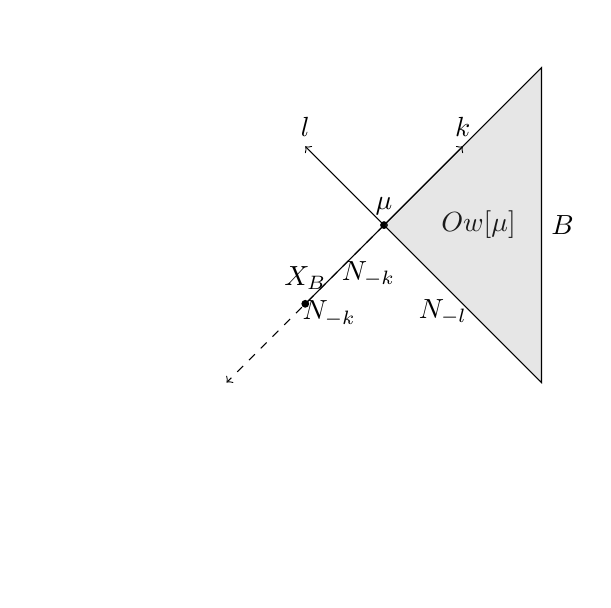
\begin{tikzpicture}
  \coordinate (bl) at (0, 0);
  \coordinate (br) at (6, 0);
  \coordinate (tr) at (6, 7);
  \coordinate (tl) at (0, 7);
  \coordinate (x) at (3, 3.5);
  \coordinate[label=above:$\mu$] (mu) at (4, 4.5);
  \coordinate[label=above:$k$] (klab) at (5, 5.5);
  \coordinate[label=above:$l$] (llab) at (3, 5.5);
  \coordinate[label=right:$B$] (blab) at (6, 4.5);
  \coordinate[label={[label distance=-2.5mm, sloped] below left:$N_{-l}$}] (Nl) at (5, 3.5);
  \node (0) at (5.2, 4.5){$Ow[\mu]$};
  \coordinate (owtr) at (6, 6.5);
  \coordinate (owbr) at (6, 2.5);
  \coordinate (muh) at (2, 2.5);
  \coordinate (iwbl) at (0, 0.5);
  \coordinate (iwtl) at (0, 4.5);

  \draw[opacity=0] (bl) to (tl);
  \draw[opacity=0] (br) to (tr);

  \node at (mu)[circle,fill,inner sep=1pt]{};

  \draw[fill=gray, fill opacity=0.2] (mu) to (owtr) to (owbr) -- cycle;

  \draw[->] (mu) to (klab);
  \draw[->] (mu) to (llab);

  \coordinate[label={[opacity=0]left:$\widetilde B$}] (blab) at (0, 2.5);

  \onslide<1-5> {
    \draw[->, dashed] (mu) to (muh);
    \coordinate[label={[label distance=-2.25mm] below right:$N_{-k}$}] (klabel) at (x);
  }

  \onslide<6->{
    \draw (mu) to (x);
    \node at (x)[circle,fill,inner sep=1pt,label=above:$X_B$]{};
    \coordinate[label={[label distance=-2.25mm] below right:$N_{-k}$}] (klabel) at (3.50, 4);
  }

\end{tikzpicture}
